\documentclass[12pt,onecolumn,a4paper]{article}
\usepackage{epsfig,graphicx,subfigure,amsthm,amsmath}
\usepackage{algpseudocode}
\usepackage{color,xcolor}     
\usepackage{xepersian}
\settextfont[Scale=1.2]{BZAR.TTF}
\setlatintextfont[Scale=1]{Times New Roman}

\renewcommand{\baselinestretch}{1.5}

\begin{document}
\makebox[10cm][c]{
\begin{minipage}{10cm}
	\centering
	
\includegraphics[height=4cm]{ut.png}
\end{minipage}
\begin{minipage}{5cm}
	\begin{center}
	\begin{persian}
        {\Large \bfseries به نام خدا \\}
        \hspace{5cm}
		{\large \bfseries دانشگاه تهران \\}
		{\large \bfseries پردیس دانشکده های فنی \\}
		{\normalsize \bf دانشکده مهندسی برق و کامیپوتر }
	\end{persian}
	\end{center}
\end{minipage}
\begin{minipage}{7cm}
	\centering
	
\includegraphics[height=4cm]{fanni.png}
\end{minipage}
}

\begin{center}
    \vskip 1.5cm
    \vspace{2cm}
    {\huge\titlefont\bfseries گزارش نهایی}\par
    \vspace{1cm}
    {\large\bfseries{درس یادگیری ماشین}}
    \\
    \vspace{2cm}
    {\normalsize\bfseries{ امیرحسین عباسکوهی \hspace{0.3cm} 810197539}}
    \vskip 5mm
    {\normalsize\bfseries{آرش رسولی \hspace{1.4cm} 810197515}}
    \vskip 5mm
    {\normalsize\bfseries{نازنین یوسفیان \hspace{1.2cm} 810197610 }}
    \vskip 5mm
    {\normalsize\bfseries{حمید خدادادی \hspace{1.2cm} 810197499}}
    
    \vspace{3cm}
    
    پاییز 1400
\end{center}


% \title{عنوان مقاله} 
% \author{میلاد رفیعی، کارشناسی دانشگاه علم وصنعت ایران واحد بهشهر\\
% دانشجوی کارشناسی ارشد دانشگاه تفرش\\
% مهندسی صنایع}
% \date{\today}
% \maketitle

\section{مقدمه} 

ما در این پروژه قصد داریم که یک الگوریتم یادگیری ماشین را به هدف تحلیل و پردازش، طبقه بندی و خوشه بندی داده ها، روی مجموعه بزرگی از داده های "موسیقی محلی ایرانی" اجرا کنیم.
در ابتدا برای انجام این کار به جمع آوری داده ها پرداختیم

پس از مرحله جمع آوری داده، در این مرحله مدل های مختلف طبقه بندی و خوشه بندی را بر روی داده های جمع آوری شده توسط کل کلاس آزمون کردیم که نتایج آن در این گزارش بحث خواهد شد.

\section{تمیز سازی داده ها}
در دیتاست اصلی برخی از آهنگ ها هستند که \lr{header} های آن ها به درستی نوشته نشده اند و هنگام خوانده شدن توسط توابع مخصوص پایتون دچار مشکل می شوند. به همین دلیل ما این آهنگ ها که تعداد آنها ۵ عدد (۲ عدد در دسته لری، ۲ عدد در دسته ترکی و یک عدد در دسته بندری) بود را شناسایی کردیم و از رده داده ها خارج کردیم.

داده های پروژه در قالب فایل های \lr{mp3} داده شده اند. از آن جایی که استخراج ویژگی های عددی از یک فایل صوتی توسط کتابخانه \lr{librosa} بر روی فایل های \lr{wav} انجام می شود، نیاز است تا فایل های صوتی خود را به این فرمت تبدیل کنیم. همچنین این یک فرمت بسیار \lr{loss less} است، به این معنی که نزدیکترین نمایش دیجیتال از صدای اصلی را بدون کاهش قابل توجه کیفیت صدا را ضبط می‌کند؛ در حالی که داده در فرمت \lr{mp3} به صورت فشرده ذخیره می‌شود تا بتوان آن را راحت تر و هر چند با کیفیت پایین‌تر توزیع کرد.

سیگنال صوتی یک سیگنال سه بعدی است که در آن سه محور زمان، دامنه و فرکانس را نشان می‌دهد(شکل\ref{fig:Acoustic signal} ).

\begin{figure}
  \centering
  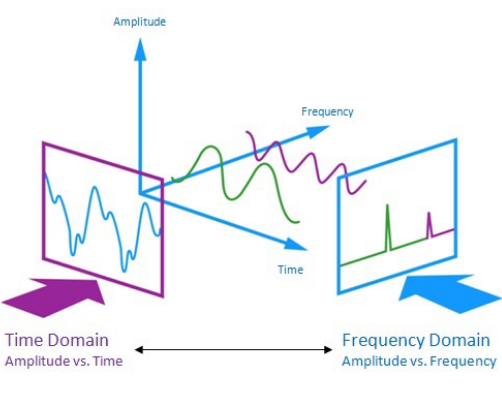
\includegraphics[width=10cm,height=7cm,keepaspectratio]{1.png}
  \caption{محور های یک سیگنال صوتی}
  \label{fig:Acoustic signal}
\end{figure}

همانطور که گفته شد، یکی از ابعاد سیگنال های صوتی، زمان است؛ ویژگی هایی که قرار است برای هر آهنگ استخراج شود، در فریم های مختلف (در طول زمان) داده هستند.
هر ثانیه در حدود ۴۳ فریم می‌باشد. طبیعتاَ نگهداری این همه ویژگی زیاد کار معقولانه ای نیست و به مشکلات زیادی از جمله کمبود حافظه، کمبود داده و نحسی ابعاد (\lr{Curse of dimensionality}) بر می‌خوریم و همچنین این داده ها اطلاعات خیلی مفیدی هم به ما نخواهند داد.

برای رفع این مشکل تصمیم گرفته شد که  به هر ویژگی ای که در فریم های مختلف ارائه می‌شود، به عنوان یک توزیع
گاوسی نگاه کنیم و میانگین و واریانس آن را به عنوان یک فیچر در نظر بگیریم.

حال مشکل دیگری که به وجود می‌آمد این بود که اگر بخواهیم ویژگی ها را در کل طول آهنگ بخوانیم و میانگین بگیریم ممکن بود بخش زیادی از داده را از دست بدهیم. به همین دلیل ما هر آهنگ را به بخش‌های کوچکتر ۳۰ ثانیه ای شکاندیم و ویژگی ها در در طول آن ۳۰ ثانیه درآوردیم و توزیع گاوسی آن را جزو فیچر هایمان در نظر گرفتیم. 

همچنین در فرآیند شکستن آهنگ ها، از هر فایل داده، ۳۰ ثانیه را از ابتدا و انتهای آن آهنگ حذف می‌کنیم. چون به طور معمول، ابتدا و انتهای آهنگ ها دارای اطلاعات خاصی نیستند و اغلب با گوش دادن به ۱۰ یا ۱۵ ثانیه ابتدایی و انتهایی یک آهنگ، نمی توان در مورد آن زیاد اظهار نظر کرد.


\section{ویژگی های یک سیگنال صوتی}
برای حل مسئله که ساختن یک مدل برای طبقه بندی کردن موسیقی های محلی است باید از داده های موجود استفاده کنیم. هر سیگنال صوتی دارای ویژگی های بسیاری است که ما در اینجا به معرفی چند تا از آن هایی که در پروژه خود استفاده می‌کنیم، می‌پردازیم.

\begin{itemize}
    \item[*] \lr{Zero Crossing Rate}: نرخ عبور صفر، نرخ تغییرات علامت در طول یک سیگنال است؛ یعنی نرخی که در آن، سیگنال از مثبت به منفی یا به صورت برعکس تغییر می کند. این ویژگی، هم در تشخیص گفتار و هم در بازیابی اطلاعات موسیقی به شدت مورد استفاده قرار گرفته است. در عکس زیر بخشی از سیگنال یک آهنگ از هر دسته را میبینیم که \lr{Zero Crossing} های آن مشخص شده است(شکل \ref{fig:ZeroCrossing}).
    
    \item[*] \lr{Spectral Centroid} (مرکز طیفی): این ویژگی نشان می دهد که مرکز جرم برای یک داده صوتی در کجای آن قرار دارد. و از طریق میانگین وزنی فرکانس های موجود در داده صوتی محاسبه می شود. اگر فرکانس‌های موسیقی در طول آهنگ یکسان باشند، مرکز طیفی، حول یک مرکز خواهد بود؛ و اگر فرکانس‌های بالایی در انتهای داده صوتی وجود داشته باشد، مرکز به سمت انتهای آن متمایل می‌شود(شکل \ref{fig:SpectralCentroid}). 
    
    \begin{equation}
        Centroid = \frac{\sum_{n=0}^{N-1}f(n)x(n)}{\sum_{n=0}^{N-1}x(n)}
    \end{equation}
    
    \item[*] \lr{Spectral Rolloff}: ین ویژگی، بیانگر فرکانس قسمت هایی از سیگنال است که کمتر از درصد مشخصی از کل انرژی طیفی هستند(شکل \ref{fig:SpectralRolloff}).
    
    \item[*] \lr{Chroma Frequencies}: ویژگی‌های کروما یک نمایش جالب و قدرتمند برای داده صوتی است که در آن کل طیف در 12 تا \lr{bin} نمایش داده می‌شود. که نشان‌دهنده 12 نیم‌تون (یا کروما) متمایز اکتاو موسیقی است.
از آنجایی که در موسیقی، نت‌هایی که دقیقاً یک اکتاو از هم فاصله دارند بسیار شبیه یکدیگر هستند، دانستن توزیع کروما حتی بدون فرکانس مطلق (یعنی اکتاو اصلی) هم می‌تواند اطلاعات مفیدی در مورد داده صوتی بدهد. و حتی ممکن است شباهت هایی را آشکار کند که در طیف اصلی مشخص نیست.
در هر فریم، \lr{pitch} های متفاوت وجود دارد که کیفیت یک لحن خاص را از بقیه صداهای داخل یک اکتاو جدا می کند و تفاوت های ادراکی گام ها در یک اکتاو و یکسانی ادراکی گام هایی که با یک یا چند اکتاو کامل از هم جدا شده اند را توصیف می کند(شکل \ref{fig:ChromaFreq}).

    \item[*] \lr{Mel Frequency Cepstral Coefficients (MFCC)s}: این ویژگی یکی از مهم ترین روش ها برای استخراج ویژگی سیگنال صوتی است و به طور عمده در هنگام کار بر روی سیگنال های صوتی استفاده می شود. \lr{MFCCs} یک سیگنال مجموعه کوچکی از ویژگی ها (معمولاً حدود 10-20) هستند که به طور خلاصه شکل کلی یک پوشش طیفی را توصیف می کنند(شکل \ref{fig:MFCC}).
    
\end{itemize}

\begin{figure}
  \centering
  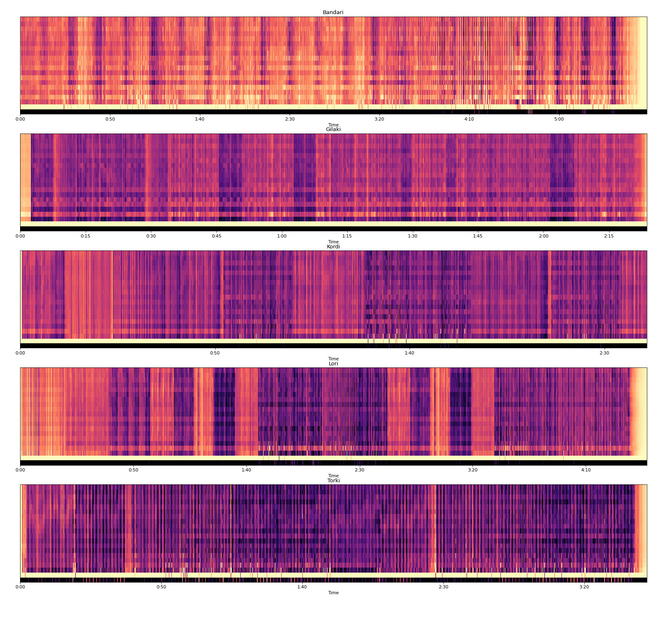
\includegraphics[width=14cm,height=10cm,keepaspectratio]{6.png}
  \caption{بررسی ویژگی \lr{MFCC} بر روی هر دسته موسیقی}
  \label{fig:MFCC}
\end{figure}

\begin{figure}
  \centering
  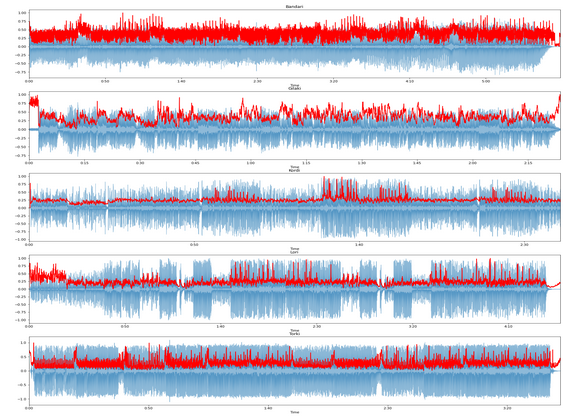
\includegraphics[width=12cm,height=8cm,keepaspectratio]{3.png}
  \caption{بررسی ویژگی \lr{Spectral Centroid} بر روی هر دسته موسیقی}
  \label{fig:SpectralCentroid}
\end{figure}

\begin{figure}
  \centering
  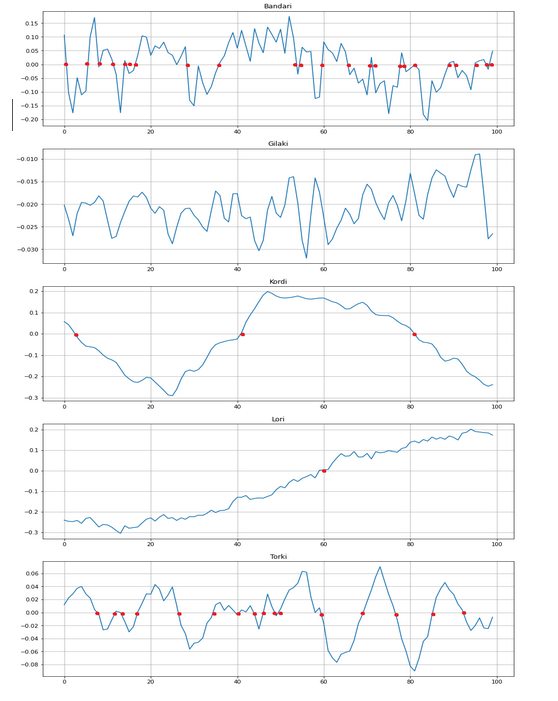
\includegraphics[width=23cm,height=18cm,keepaspectratio]{2.png}
  \caption{بررسی ویژگی \lr{Zero Crossing} بر روی هر دسته موسیقی}
  \label{fig:ZeroCrossing}
\end{figure}

\begin{figure}
  \centering
  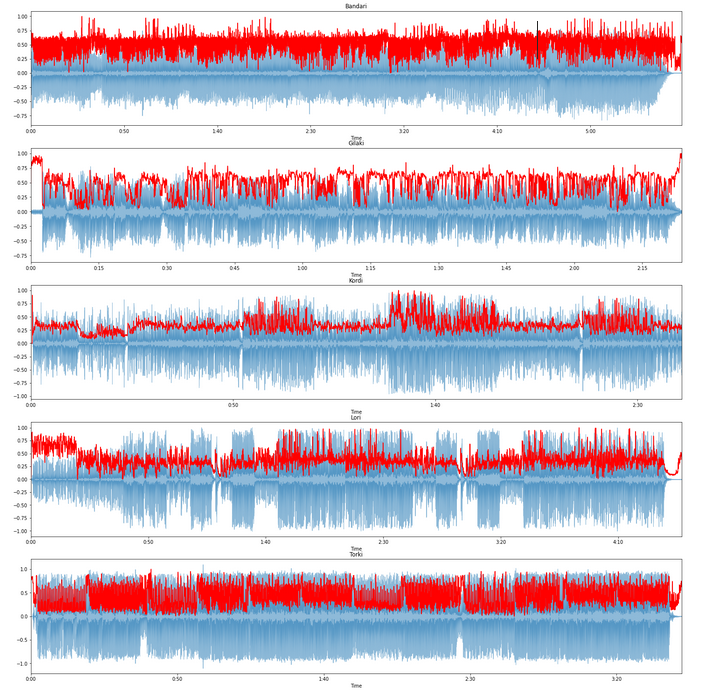
\includegraphics[width=20cm,height=15cm,keepaspectratio]{4.png}
  \caption{بررسی ویژگی \lr{Spectral Rolloff} بر روی هر دسته موسیقی}
  \label{fig:SpectralRolloff}
\end{figure}

\begin{figure}
  \centering
  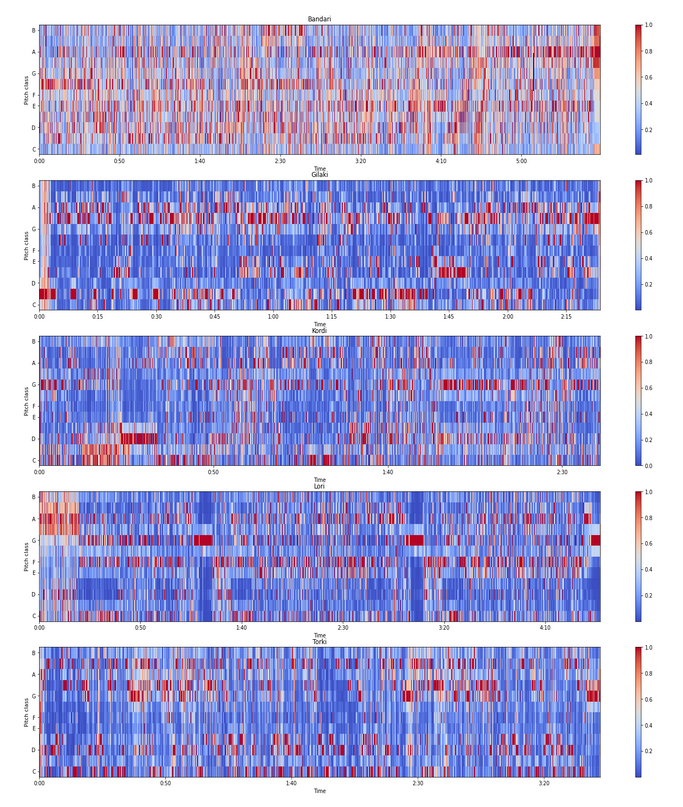
\includegraphics[width=20cm,height=15cm,keepaspectratio]{5.png}
  \caption{بررسی ویژگی \lr{Chroma Frequencies} بر روی هر دسته موسیقی}
  \label{fig:ChromaFreq}
\end{figure}

\section{استخراج ویژگی ها}
در بخش قبل ویژگی های مختلف یک سیگنال صوتی معرفی شدند.
حال ما نحوه ی استخراج و تعداد ویژگی های خود را در این قسمت ذکر می کنیم.

نکته اول که منظور از هر پارت در اینجا، قسمت های ۳۰ ثانیه ای هستند که آهنگ ها به آن ها تقسیم شده اند.
نکته بعدی این است که هر ثانیه در حدود ۴۳.۱  فریم می باشد؛ در نتیجه یک پارت ۳۰ ثانیه ای دارای ۱۲۹۳ تا فریم است.

برای رسیدن به ویژگی های یک سیگنال صوتی، برای هر پارت به صورت جداگانه از 5 ویژگی \lr{Zero Crossing Rate}، \lr{Spectral Centroid}، \lr{Spectral Rolloff}، \lr{Chroma Frequencies} و \lr{MFCC} استفاده کردیم.

در \lr{Zero Crossing Rate} مجموع آن‌ها در طول کل فریم های یک پارت را حساب کرده و به عنوان یک ویژگی در نظر می‌گیریم. پس در نهایت به ما 1 ویژگی خواهد داد.

در \lr{Spectral Centroid}  این ویژگی در ۱۲۹۳ تا فریم حساب می شود؛ که آن را یک توزیع گاوسی فرض می کنیم و میانگین و واریانس آن را به ویژگی ها در نظر می گیریم. پس در نهایت به ما 2 ویژگی خواهد داد.

در \lr{Spectral Rolloff}،  این ویژگی در ۱۲۹۳ فریم حساب می شود؛ که آن را یک توزیع گاوسی فرض می کنیم و میانگین و واریانس آن را به ویژگی ها در نظر می گیریم. در نتیجه به 2 ویژگی در اینجا می رسیم.

در \lr{Chroma Frequencies} این بخش دارای ۱۲ ویژگی است که  در ۱۲۹۳ فریم حساب می شود؛ همانطور که قبل تر هم اشاره شد، برای هر یک از آنها یک توزیع گاوسی فرض می کنیم و میانگین و واریانس آن را به ویژگی ها در نظر می گیریم. پس در نهایت ۱۲ تا میانگین و ۱۲ تا واریانس داریم. در اینجا به 24 ویژگی می رسیم.

در \lr{MFCCs} ین بخش دارای ۲۰ ویژگی است که  در ۱۲۹۳ فریم حساب می شود؛ که برای هر یک از آنها یک توزیع گاوسی فرض می کنیم و میانگین و واریانس آن را به ویژگی ها در نظر می گیریم. پس در نهایت ۲۰ تا میانگین و ۲۰ تا واریانس داریم. در این بخش هم بخ 40 ویژگی می رسیم.

پس در کل برای هر پارت 69 ویژگی داریم و این ویژگی ها را در یک فایل \lr{csv} به همراه \lr{label} آن ها ذخیره می کنیم و در ادامه برای مدل های مختلف از این فایل استفاده خواهیم کرد.

\section{نرمالایز کردن داده ها}
در اولین گام پس از خواندن دیتا و جدا کردن دیتای فیچر ها از دیتای لیبل ها، اقدام به نرمال کردن دیتای فیچر ها کردیم. برای این کار از \lr{MinMaxScaler} کتابخانه \lr{sklearn} استفاده کردیم. این الگوریتم دیتا را استانداردسازی می کند. یعنی به صورتی تغییر می دهد که داده ها دارای توزیع گاوسی شوند و میانگین صفر و واریانس یک بگیرند. ما رنج کمینه و بیشینه استانداردسازی را 0 و 1 قرار دادیم تا داده ها نرمال هم بشوند و در محدوده بین صفر و یک قرار بگیرند. این کار باعث می شود که وزن همه داده ها با هم برابر شود و اثر یکی بر دیگری برتری نداشته باشد؛ این کار باعث می شود که مدل ما با داده ها به صورت \lr{fair} رفتار داشته باشد. اگر داده های فیچر ما مقدار بزرگی داشته باشند و \lr{scale} بیشتری را شامل شوند، باعث می شود که تاثیر بیشتری روی انتخاب برچسب یک کلاس داشته باشند؛ حال اگر آن فیچر با آن لیبل ناسازگار باشد و تاثیر نامطلوبی در انتخاب آن لیبل بگذارد، و اگر هم مقدار \lr{scale} بزرگی داشته باشد، آموزش مدل ما را با مشکل رو به رو خواهد کرد.

الگوریتمی که از آن برای نرمال کردن داده ها استفاده کردیم بدین صورت است که همه داده های فیچر ها را از کمترین داده آن فیچر کم می کند و حاصل را بر اختلاف بزرگترین داده آن فیچر از کوچک ترین داده آن فیچر، تقسیم می کند.

به طور خلاصه تاثیر این کار این است که مدل را از سوگیری روی فیچری از دیتا نجات می دهد، حجم محاسبات عددی را بسیار کاهش می دهد (به خصوص در محاسبه گرادیان نزولی در شبکه های عصبی) و سرعت مدل را بسیار بهبود می بخشد و در نهایت دقت بهتری را برای مدل نتیجه می دهد.

\section{انتخاب برترین زیر مجموعه از ویژگی ها}

فیچر های داده‌ای که برای آموزش مدل‌های یادگیری ماشین خود استفاده می‌کنیم تاثیر زیادی بر عملکردی که از مدل خود بدست می آوریم دارد. با \lr{feature selection} می توانیم عملکرد مدل را بهبود ببخشیم، سرعت آموزش مدل را افزایش دهیم و \lr{overfit} شدن مدل را به عقب بیندازیم. همچنین از نحسی ابعاد برای مدل خود جلوگیری کنیم. (این مسئله بیان می کند که اگر تعداد ابعاد داده ما بالا باشد یا به عبارتی تعداد فیچر های بالایی داشته باشد، آنگاه به دیتای بیشتری برای آموزش مدل خود نیاز داریم تا \lr{overfitting} رخ ندهد؛ در غیر این صورت عملکرد مدل با مشکل روبرو خواهد شد.)

برای این هدف، نیاز بود تا فیچر هایی که در انتخاب برچسب کلاس یک داده، تاثیر نامطلوب یا حتی تاثیر کمی می گذارند را حذف کنیم. برای این کار در ابتدا همبستگی میان فیچر های مختلف و لیبل را در نظر گرفتیم.
سپس \lr{heatmap} این همبستگی بین فیچر های مختلف و لیبل آن دیتا را رسم کردیم.

همبستگی بین دو متغیر می‌تواند مثبت باشد (افزایش مقدار فیچر، احتمال انتخاب متغیر هدف را افزایش می‌دهد.) یا منفی (افزایش مقدار فیچر، احتمال انتخاب متغیر هدف را کاهش می‌دهد.) و \lr{heatmap} تشخیص اینکه کدام ویژگی‌ها بیشتر به متغیر هدف مرتبط هستند را آسان می‌کند.

قبل از آن که این \lr{heatmap} را رسم کنیم، از داده ها لگاریتم گرفتیم، بدین منظور که ممکن است فیچر ها و لیبل ها، همبستگی نمایی داشته باشند و با لگاریتم گرفتن می توانیم همبستگی خطی بین آن ها را ببینیم. 

از \lr{heatmap} می توانیم نتیجه بگیریم که اگر چند فیچر نسبت به همدیگر همبستگی بالایی دارند، آن گاه یکی از آن فیچر ها را برای انتخاب لیبل داده استفاده کنیم و با این کار کار مدل سازی را ساده تر کنیم و از لحاظ زمانی، مدل را بهبود ببخشیم و آن را به محاسبات کم فایده مشغول نکنیم. یا اگر فیچری در انتخاب لیبل یک داده، اثر کمی دارد یا حتی اثر نامطلوبی دارد، آن گاه آن را از لیست فیچر ها برای انتخاب برچسب داده حذف کنیم.

در آخر این بخش، 50 تا از بهترین فیچر ها برای تخمین متغیر هدف را پس از سورت کردن میزان همبستگی بین فیچر ها و لیبل داده، نمایش دادیم.

در ادامه، از روش دیگر \lr{feature selection} سعی کردیم که عملیات بالا را تکرار کنیم.
فرآیند \lr{feature selection} یا انتخاب ویژگی، فرآیند کاهش تعداد متغیرهای ورودی برنامه، هنگام توسعه و پیاده سازی یک مدل پیش‌بینی است.کاهش تعداد متغیرهای ورودی برای کاهش هزینه محاسباتی مدل سازی و در برخی موارد برای بهبود عملکرد مدل دلخواه است. روش‌های انتخاب ویژگی مبتنی بر آمار، شامل ارزیابی رابطه بین هر متغیر ورودی و متغیر هدف با استفاده از آمار و انتخاب آن دسته از متغیرهای ورودی است که قوی‌ترین رابطه را با متغیر هدف دارند. این روش ها می توانند سریع و موثر باشند؛ اگرچه انتخاب معیارهای آماری به نوع داده متغیرهای ورودی و خروجی بستگی دارد.

هدف از عملیات انتخاب ویژگی از بین کل ویژگی ها، این است که آن ویژگی هایی را انتخاب کنیم که مطمئن هستیم به ما در آموزش مدل کمک خواهند کرد و بار اضافی به مدل ما تحمیل نمی کنند و برای آموزش مدل ما مفید هستند.
ما در این فرآیند در اولین گام، آن دسته از ویژگی هایی از دیتا که برای مدل سازی ما مفید نیستند و بار محاسباتی اضافی و بدون فایده به مدل ما وارد می کنند را حذف می کنیم. 

همانطور که گفته شد ما برای دیتاهای خود، 69 ویژگی مختلف در نظر گرفتیم؛ که بسیاری از این ویژگی ها باعث کند شدن فرآیند آموزش مدل ما می شدند و نگهداری آن ها هم بار زیادی به حافظه سیستم ما وارد می کرد. اما دلیل اصلی ای که باعث شد ما به این فکر بیفتیم که تعداد ویژگی های خود را کاهش دهیم، این بود که در ابتدای کار \lr{heatmap} همبستگی ویژگی های دیتاها را رسم کردیم. سپس چند ویژگی را که طبق این نقشه به لیبل داده، همبستگی کمتری داشتند و به بیانی دیگر، این ویژگی ها از یکدیگر استقلال بیشتری داشتند را انتخاب کردیم و از لیست فیچر ها حذف کردیم و سپس مدل خود را روی این داده ها اجرا کردیم. 
متوجه شدیم که در این اجرا، در مقایسه با آن که مدل را روی کل ویژگی هایش آموزش دهیم، به دقت بیشتری می توانیم برسیم. همین موضوع باعث شد که به این فکر بیفتیم که بهترین و بهینه ترین ویژگی های این داده ها را پیدا کنیم و مدل خود را روی این ویژگی ها از داده ها آموزش دهیم.
یعنی به طور خلاصه، انگیزه اصلی ما این بود که عملکرد برخی از مدل‌ها در صورت گنجاندن متغیر های ورودی که به متغیر هدف ما کمتر مرتبط بودند، کاهش می یافت.
نکته دیگری که پس از مطالعه منابع مختلف در یافتیم آن بود که وجود متغیرهای غیر اطلاعاتی، می‌تواند عدم قطعیت را به تخمین های مدل ما اضافه کند و اثربخشی کلی مدل را کاهش دهد.

به طور کلی دو نوع عملکرد برای انتخاب ویژگی داریم؛ بدون نظارت و با نظارت.
در انتخاب ویژگی بدون نظارت، از متغیر هدف یا همان لیبل کلاس آن دیتا استفاده نمی کنیم و سعی می کنیم که ویژگی های اضافی را حذف کنیم که در این جا می توان از مفهوم همبستگی بین ویژگی ها استفاده کرد. و در انتخاب ویژگی با نظارت، از متغیر هدف یا همان لیبل کلاس آن دیتا استفاده می کنیم و سعی می کنیم که ویژگی های نامربوط به آن لیبل را حذف کنیم. 

سه فایده ای که می توان برای استفاده از فرآیند انتخاب ویژگی برشمرد این است که:

\vspace{10}

1- کاهش \lr{overfitting}: وقتی ویژگی هایی که تاثیر کم یا حتی تاثیر منفی در عملکرد تخمین زدن مدل ما را دارند را در نظر نمی گیریم، در واقع از آن که مدل ما روی داده های نویزی \lr{fit} شود جلوگیری کرده ایم و این کار از \lr{overfitting} جلوگیری خواهد کرد.

2- افزایش دقت: منطقی است که وقتی تمرکز مدل خود را روی آموزش روی ویژگی هایی از داده قرار دهیم که عملکرد مدل بهبود یابد، آنگاه دقت تخمین مدل هم افزایش خواهد یافت.

3- کاهش زمان آموزش: چیزی که به وضوح به آن برخوردیم این بود که سرعت آموزش مدل ما، وقتی که تعداد ویژگی های دیتا را کاهش می دادیم، بسیار افزایش می یافت؛ که ناشی از کم شدن بار محاسباتی آموزش مدل است.

\vspace{10}

یزی که از آن برای پروژه خود استفاده کردیم، روش \lr{univariate selection} از کتابخانه \lr{sklearn} بود.

این کتابخانه، برای انتخاب ویژگی هایی که قوی ترین رابطه را با متغیر هدف یا همان لیبل کلاس هدف دارند، کلاس \lr{SelectKBest} را ارائه می دهد که می تواند با مجموعه ای از آزمون های آماری مختلف برای انتخاب تعدادی دلخواه از ویژگی ها استفاده شود.

در ابتدای کار، مدل را با استفاده از کلاس \lr{SelectKBest} تعریف می کنیم. برای طبقه‌بندی، روش \lr{«chi2»} را به‌عنوان تابع امتیازدهی تنظیم می‌کنیم. تعداد هدف ویژگی ها با پارامتر \lr{k} تعریف می کنیم. سپس الگوریتم را بر روی داده های آموزش و لیبل آن ها، برازش و تبدیل می کنیم.

\begin{equation}
        \chi^2 = \sum \frac{(O_i - E_i)^2}{E_i} ; O_i: observed value, E_i: expected value
\end{equation}

این کلاس \lr{SelectKBest}، روش آماری \lr{«chi2»} را بین هر یک از ویژگی های غیر منفی و لیبل کلاس محاسبه کند. این امتیاز می‌تواند برای انتخاب \lr{n} تا ویژگی‌ با بالاترین مقادیر برای آماره مجذور \lr{«chi»} استفاده شود. این روش وابستگی بین ویژگی ها را اندازه گیری می کند، بنابراین با استفاده از این تابع ویژگی هایی که به احتمال زیاد مستقل از لیبل کلاس هستند و بنابراین برای طبقه بندی نامربوط هستند در نظر گرفته نمی شوند.

تعداد \lr{k} یا تعداد هدف ویژگی ها را چند عدد مختلف قرار دادیم و تاثیر آن ها را با آموزش مدل طبقه بند \lr{MLP} سنجیدیم. از مقدار \lr{k} برابر 10 و 15 و 20 شروع کردیم و 40 و 40 و 60 را هم امتحان کردیم. بهترین مقداری که برای هایپرپارامتر \lr{k} نتیجه گرفتیم مقدار 50 تا از بهترین فیچر ها از بین کل 69 فیچر بود. و سپس با استفاده از متد \lr{get\_feature\_names\_out}، نام این 50 فیچر برتر را نگهداری کردیم تا در آموزش مدل های خود از آن ها استفاده کنیم.
در انتهای این بخش، فیچر های برتری که توسط الگوریتم \lr{feature selection} انتخاب شده بودند را با فیچر های برتری که توسط \lr{heatmap correlation} انتخاب شده بودند را مقایسه کردیم. 

مشاهده کردیم که از 50 تا فیچر، این دو الگوریتم در 14 تا فیچر متفاوت بودند؛ که ما فیچر های انتخابی توسط الگوریتم \lr{feature selection} را برای مدل سازی خود در ادامه استفاده کردیم.

\section{جداسازی داده آموزش و آزمون}
تقسیم کردن دیتا به دو بخش دیتای آموزش و دیتای آزمون، تکنیکی برای ارزیابی عملکرد یک الگوریتم یادگیری ماشین است. ما با این روش و نتایج حاصل از آن، به ارزیابی عملکرد الگوریتم های ماشین لرنینگ مختلف می پردازیم. این روش زمانی مناسب است که مجموعه داده ها به اندازه کافی بزرگ باشد؛ یا مدل ما مدلی مهم و پر هزینه باشد و نیاز داشته باشیم که به صورت حتمی آن را آزموده باشیم و از صحت عملکرد آن اطمینان حاصل کرده باشیم. ما با این روش، مدل خود را روی داده های آموزش اجرا می کنیم و \lr{fit} می کنیم و مدل خود را دیگر روی داده آزمون، \lr{fit} نمی کنیم. سپس با اجرای مدل خود روی داده آزمون، عملکرد مدل خود را می سنجیم. با این کار تا حدی خوبی اطمینان حاصل می کنیم که اگر در آینده، دیتای جدیدی که لیبل ندارد به مدل ما داده شود، با دقت خوبی می تواند برچسب آن را حدس بزند.

درصد تقسیم بهینه ای برای داده آموزش و آزمون وجود ندارد و به صورت تجربی بدست می آید.
ما باید با توجه به هدف و نوع مدل خود، هزینه های محاسباتی در آموزش مدل و هزینه های محاسباتی در ارزیابی مدل، این درصد را محاسبه کنیم.

و نکته دیگر اینکه، داده های آموزش و داده های آزمون باید جامعیت خوبی از کل دیتا داشته باشند و به صورت تصادفی انتخاب شده باشند و بهتر است که بالانس و \lr{fair} از لحاظ تعداد داده های هر برچسب باشند.

باید مقدار داده های آموزش و آزمون به حدی باشد که از طرفی داده برای آموزش مدل کم نیاید و دچار نحسی ابعاد نشویم و از طرفی داده آموزش آنقدر زیاد نباشد که مدل ما روی داده های نویزی هم آموزش ببیند؛ به صورت خلاصه، میزان داده ها باید به گونه ای باشد که مدل ما \lr{overfit} و \lr{underfit} نکند.

ما از الگوریتم \lr{train\_test\_split} کتابخانه \lr{sklearn} استفاده کردیم و به طور تجربی و با چند بار تلاش به میزان 80 درصد داده ها را برای آموزش مدل اختصاص دادیم و 20 درصد داده ها را هم برای آزمون مدل خود جدا کردیم.

همچنین در دو \lr{plot bar} مختلف، بالانس بودن تقریبی تعداد دیتا های هر کلاس در مجموعه دیتای آموزش و آزمون را نشان دادیم.(شکل \ref{fig:TestTrain})

\begin{figure}
  \centering
  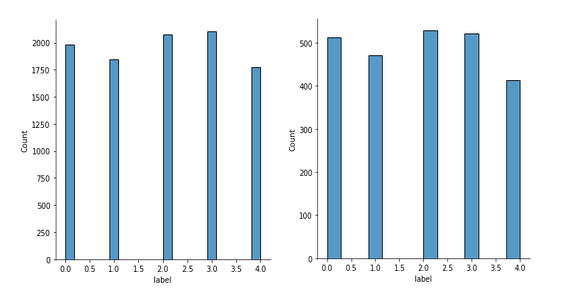
\includegraphics[width=10cm,height=7cm,keepaspectratio]{7.png}
  \caption{تعداد داده های هر دسته در مجموعه داد های تمرین و آزمون}
  \label{fig:TestTrain}
\end{figure}

\section {کاهش ابعاد داده ها}
در ادامه نیاز داشتیم که ابعاد داده ها کاهش دهیم تا هم الگوریتم های خوشه بندی به خوبی اجرا شوند و هم بتوانیم دیتا را \lr{visualize} کنیم. برای این کار از الگوریتم کاهش ابعاد \lr{PCA} یا  \lr{Principal Component Analysis} استفاده کردیم. این روش از عملیات های ماتریسی ساده جبر خطی و آمار برای محاسبه \lr{projection} داده های اصلی به همان ابعاد داده یا داده با ابعاد کمتر استفاده می کند. این روش ماهیت اصلی داده ها را حفظ می کند ولی کمک می کند که لیبل داده ها را در فضای فرعی با تعداد فیچر های کمتر و ابعاد پایین تر تخمین بزنیم.

این روش بدین صورت عمل می کند که در ابتدا میانگین هر ستون فیچر را ار داده های آن ستون کم می کند؛ این کار باعث می شود که کار محاسبات ساده تر بشود.

\begin{equation}
        x_j^{(i)} = \frac{x_j^{(i)-\bar{x_j}}}{\sigma_j} \forall{j}
\end{equation}

سپس نیاز است تا حاصل ضرب ماتریس داده ها در وارونش را بدست بیاوریم. برای این کار می توانیم از معادل این عملیات یعنی محاسبه ماتریس کوواریانس استفاده کنیم. همبستگی یک معیار نرمال شده از مقدار و جهت (مثبت یا منفی) است که دو ستون با هم تغییر می کنند. کوواریانس یک نسخه تعمیم یافته از همبستگی چندین ستون است. در ادامه طبق محاسبات لاگرانژ، نیاز است که مقدار ویژه و بردار ویژه را برای حاصل ضرب ماتریس داده ها در وارونش را محاسبه کنیم. رابطه های زیر از لکچر های درس \lr{cs229} دانشگاه استنفورد آورده شده است.

\begin{equation}
    max \hspace{10} \frac{1}{m}\sum_{i=1}^{m}(x^{(i)^T}u)^2 ; s.t ||u||=1
\end{equation}

\begin{equation}
    L(u, \lambda)=u^T \Sigma u-\lambda(u^Tu-1)
\end{equation}

\begin{equation}
    max \hspace{10} u^T(\frac{1}{m}\sum_{i=1}^{m}x^{(i)}x^{(i)^T})u = u^T \Sigma u ; ||u^Tu||=1
\end{equation}

\begin{equation}
    \frac{\partial L}{\partial u} = u^T \Sigma - \lambda u = 0
\end{equation}

\begin{equation}
    \frac{\partial L}{\partial \lambda} = u^T u - 1 = 0
\end{equation}

بردارهای ویژه، جهت ها یا \lr{component} های زیرفضای کاهش یافته را نشان می دهند، در حالی که مقادیر ویژه، نشان دهنده مقدار بزرگی برای آن جهت ها هستند. حال بردارهای ویژه را بر اساس مقادیر ویژه به ترتیب نزولی مرتب می کنیم، و سپس به تعداد \lr{component} ها از بردارهای ویژه انتخاب می‌کنیم که مولفه‌های اصلی فضای فرعی جدید هستند و بزرگترین مقادیر ویژه را دارند. ما در این قسمت از الگوریتم \lr{PCA} کتابخانه \lr{sklearn} استفاده کردیم و تعداد \lr{component} ها را هم برابر 2 قرار دادیم. در آخر داده های ورودی را به 2 بعد کاهش داده و نمایش دادیم.

و در آخر این بخش هم، \lr{dendrogram} (نموداری است که رابطه سلسله مراتبی بین اشیا را نشان می دهد. معمولاً به عنوان خروجی از خوشه بندی سلسله مراتبی ایجاد می شود. کاربرد اصلی این نمودار یافتن بهترین تخصیص اشیا به خوشه ها است.) داده های آموزش و آزمون را در فضای فرعی جدید رسم کردیم(شکل \ref{fig:dendrogram}).

\begin{figure}
  \centering
  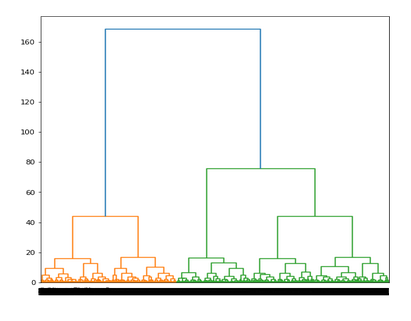
\includegraphics[width=10cm,height=7cm,keepaspectratio]{8.png}
  \caption{نمودار های \lr{dendogram} برای داده های آموزش و آزمون}
  \label{fig:dendrogram}
\end{figure}

\section{طبقه بندی}

ر ادامه در ابتدا به وسیله سه طبقه بند، به طبقه بندی داده ها پرداختیم. سه طبقه بندی که در این پروژه استفاده کردیم، طبقه بند \lr{KNN} و طبقه بند \lr{SVM} و طبقه بند \lr{MLP} هستند. سپس پس از اجرای هر مدل روی داده های آموزش و آزمون، دقت آن مدل، \lr{classification report} مربوط به آن مدل، که شامل \lr{precision} و \lr{recall} و \lr{f1-score} مربوط به هر یک از پنج لیبل کلاس ها هستند را نمایش دادیم؛ و در آخر \lr{roc curve} مربوط به آن مدل را رسم کردیم و مساحت زیر نمودار آن را به ازای هر یک از پنج کلاس، گزارش کردیم.


\subsection{طبقه بند \lr{KNN}}
الگوریتم \lr{k} نزدیکترین همسایه (\lr{KNN}) یک الگوریتم یادگیری ماشین نظارت شده است که می تواند برای حل مسائل طبقه بندی استفاده شود. الگوریتم \lr{KNN} فرض می کند که داده های کلاس های مشابه در نزدیکی هم هستند. 

ما در این قسمت از \lr{KNeighborsClassifier} از کتابخانه \lr{sklearn} استفاده کردیم.
این الگوریتم بدین صورت عمل می کند که به ازای یک داده ورودی، بر اساس متریکی مثل فاصله، فاصله یک نقطه ورودی را با سایر داده ها می سنجد. حال این فاصله ها را سورت می کند و \lr{k} تا از نزدیک ترین همسایه ها را انتخاب می کند. حال بین این \lr{k} تا همسایه، بیشترین لیبل کلاس که داده ها دارند را پیدا می کند؛ و در آخر این لیبل پر تکرار را به داده ورودی هم نسبت می دهد.

یک متریک دیگری که در \lr{KNN} ممکن است استفاده شود، متریک \lr{uniform} است. در حالتی که متریک، فاصله باشد، وزن داده ها نسبت به داده هدف بر اساس فاصله سنجیده می شود ولی در این حالت که متریک \lr{uniform} استفاده شود، همه داده ها نسبت به داده هدف، وزن برابر دارند. 

ما در این پروژه، ترجیح دادیم که متریک \lr{distance} برای طبقه بندی داده ها استفاده کنیم تا به عملکرد بهتری برسیم؛ از لحاظ زمانی هم متریک فاصله قدری بهتر جواب می داد.

متریک های فاصله مختلفی را می توان برای الگوریتم \lr{KNN} در نظر گرفت؛ ما از متریک \lr{manhattan} نتیجه خوبی برای تنظیم هایپرپارامتر های مدل گرفتیم. نکته دیگر اینکه برای الگوریتم هایی مثل \lr{KNN} که از متریک فاصله بین داده ها برای طبقه بندی آن ها استفاده می کنند، نرمال سازی داده ها از اهمیت زیادی برخوردار خواهد بود و اثرش را اینجا می گذارد.
به طور کلی انتخاب یک مقدار بزرگ برای \lr{K} باعث افزایش دقت مدل و کاهش خطای آن می شود؛ چون تعداد نمونه بیشتری را برای انتخاب لیبل یک داده اثر داده ایم. اما با این کار، وضوح مرز بین کلاس ها را کم تر کرده ایم. ما \lr{K} برابر 2 را برای مدل خود مدنظر قرار دادیم.
ما اگر مقدار \lr{K} را خیلی زیاد قرار بدهیم، مدلمان دچار \lr{underfitting} می شود و نمی تواند روی دیتا به خوبی آموزش ببیند؛ همچنین اگر مقدار \lr{K} را برابر یک مقدار خیلی کوچک قرار دهیم، آنگاه مدلمان دچار \lr{overfitting} می شود و روی داده های نویزی هم آموزش می بیند که در نتیجه روی داده آزمون به خوبی جواب نمی دهد.

تفاوت الگوریتم \lr{KNN} با الگوریتم \lr{Parzen window} این است که در \lr{KNN} ما تعداد \lr{K} تعداد داده را ثابت فرض می کنیم و پهنای باند را آنقدر افزایش می دهیم تا در یک منطقه ای در اطراف داده آزمون، \lr{K} تا همسایه نزدیکش قرار بگیرد و بر اساس لیبل این \lr{K} تا همسایه نزدیکش، لیبل این داده آزمون را پیش بینی کنیم.

\begin{equation}
    p_n(x) \cong \frac{k_n/n}{V_n}
\end{equation}

نرخ خطای \lr{KNN} بین نرخ خطای \lr{Bayes} (که حداقل مقدار ممکن است) و دو برابر نرخ خطای \lr{Bayes} است. در این رابطه مقدار \lr{c} همان تعداد کلاس های دیتاست است.

\begin{equation}
    P^* \leq P \leq P^*(2-\frac{c}{c-1}P^*) \leq 2P^*
\end{equation}

در الگوریتم \lr{KNN}، هیچ پیش فرضی در مورد داده ها وجود ندارد. پیاده سازی آن ساده است و دقت و عملکرد خوبی هم دارد. اما از طرفی از لحاظ محاسباتی، الگوریتم گران قیمتی است و همچنین نیاز دارد که حافظه به نسبت بزرگی برای ذخیره سازی داده های قبلی داشته باشد. اگر مقدار \lr{N} در این الگوریتم بزرگ باشد ممکن است که الگوریتم کند شود. و همچنین این الگوریتم نسبت به مقیاس داده ها و نیز فیچر های نامربوط خیلی حساس است.

در الگوریتم \lr{KNN}، نقاط دورافتاده نقاطی هستند که تفاوت قابل توجهی از لحاظ فاصله با بقیه نقاط داده دارند. نقاط پرت بر پیش بینی مدل تاثیر می گذارد و دقت مدل را پایین می آوردند. در نتیجه، حذف نقاط پرت قبل از استفاده از \lr{KNN} توصیه می شود. همچنین وقتی با مجموعه داده های نامتعادل و غیر بایاس سروکار داریم، مدل بایاس می شود؛ در نتیجه، بخش عمده ای از نزدیکترین همسایگان به نقطه جدید ورودی، از لیبل طبقه غالب خواهند بود که این مسئله هم بر عملکرد مدل اثرگذار است. که راه حل تغییر مقیاس برای این موضوع توصیه شده است.

سه رویکرد برای کم کردن پیچیدگی محاسبات الگوریتم \lr{KNN} وجود دارد؛ یکی \lr{computing partial distance} و یکی \lr{Pre-structuring} و دیگری \lr{Editing the stored prototypes} است.

در \lr{Pre-structuring} اینطور گفته می شود که داده های آموزش را چگونه بچینیم تا جستجوی برای محاسبات \lr{KNN} ساده تر شود. الگوریتم های مختلفی مانند \lr{kd tree} و \lr{ball tree} برای این کار وجود دارد که ما \lr{ball tree} را به کار بردیم. 

الگوریتم \lr{ball tree} در طبقه بند نزدیکترین همسایه، گره ها را در مرتبه اول عمق بررسی می کند که از سمت ریشه هم شروع می شود. در طول جستجو، الگوریتم یک صف اولویت \lr{Q} "اول بیشترین احتمال" (که اغلب با یک \lr{heap} پیاده سازی می شود.) از \lr{k} نزدیک‌ترین نقطه‌ای که تاکنون با آن مواجه شده‌ اند، نگهداری می کند. کاربرد آن در \lr{KNN} بدین صورت است که اگر الگوریتم در حال جستجوی داده ها با یک نقطه آزمون \lr{t} باشد، و قبلاً نقطه‌\lr{p} (نزدیک‌ترین نقطه به \lr{t} در بین نقاطی که تاکنون با آن مواجه شده‌ است.) را دیده باشد، آن‌گاه هر زیر درختی که \lr{ball} آن از \lr{t}، دورتر به نسبت به \lr{p} باشد را می‌توان نادیده گرفت.(شکل های \ref{fig:ROCKNN} ، \ref{fig:LCKNN} و \ref{fig:BestKKNN} )

\begin{figure}
  \centering
  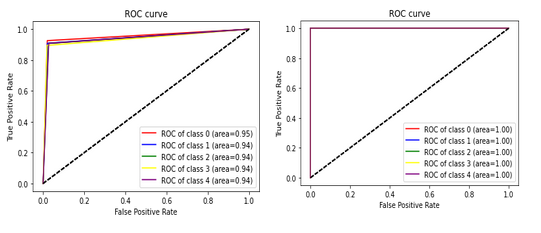
\includegraphics[width=10cm,height=7cm,keepaspectratio]{9.png}
  \caption{نمودار \lr{ROC} برای طبقه بند \lr{KNN}}
  \label{fig:ROCKNN}
\end{figure}

\begin{figure}
  \centering
  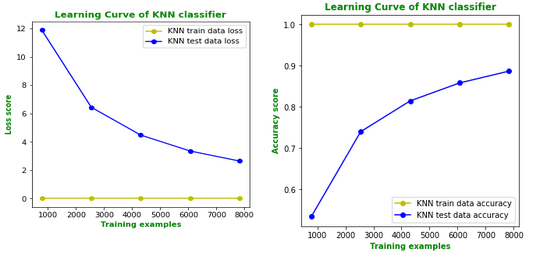
\includegraphics[width=10cm,height=7cm,keepaspectratio]{10.png}
  \caption{نمودار \lr{Learning Curve} برای طبقه بند \lr{KNN}}
  \label{fig:LCKNN}
\end{figure}

\begin{figure}
  \centering
  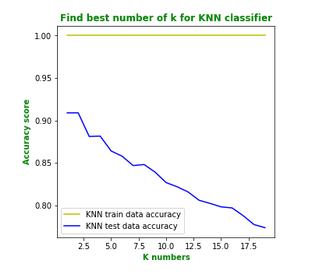
\includegraphics[width=10cm,height=7cm,keepaspectratio]{11.png}
  \caption{نمودار بهترین \lr{K} برای طبقه بند \lr{KNN}}
  \label{fig:BestKKNN}
\end{figure}

همانطور که از نمودار های این بخش هم قابل مشاهده است، دقتی که الگوریتم \lr{KNN} برای داده های آموزش به ما داده است 100 درصد و دقتی که برای داده تست به ما داده است حدود 90.8 درصد است. الگوریتم \lr{KNN}، تابع \lr{loss} ای ندارد که برای کمینه کردن آن تلاش کند. این الگوریتم روی داده ها آموزش خاصی نمی بیند و در واقع اصلاَ آموزش داده نمی شود؛ چیزی که در این الگوریتم رخ می دهد این است که یک نسخه محلی از داده ها را بخاطر می سپارد تا در حین زمان پیش بینی بتوان جستجو و پیدا کردن پرتکرار ترین لیبل آن منطقه را راحت تر پیدا کرد.
مشاهده می شود که هر چقدر تعداد داده های آموزش و تست افزایش یافته، عملکرد مدل بهتر شده است. دلیل این عملکرد این است که پایه این الگوریتم بدین صورت است که تخمین لیبل یک داده، بستگی به لیبل سایر داده های همسایه های آن داده دارد. هر چقدر که تعداد این همسایه ها بیشتر باشد، مدل بهتر و دموکراتیک تر (با توجه به لیبل های اکثریت همسایگان یک داده)، می تواند پیش بینی کند و از تخمین های نویزی جلوگیری می شود.
 همین طور در نمودار های این بخش مشاهده می کنید که تعداد بهینه \lr{k} برای این الگوریتم روی داده ها همان مقدار 2 ای که ذکر کردیم است؛ و هر چقدر که مقدار \lr{k} افزایش یافته، مقدار دقت عملکرد مدل روی داده تست کاهش یافته است.
از آن جایی که مقدار \lr{k} را هم به طور مناسب انتخاب کرده ایم، مدلمان دچار \lr{underfitting} و \lr{overfitting} نشده است.


\subsection{طبقه بند \lr{SVM}}
ماشین بردار پشتیبانی یا همان \lr{Support Vector Machines}، یک الگوریتم بر پایه روش های یادگیری با نظارت و برای طبقه بندی داده ها است.

هدف از الگوریتم ماشین بردار پشتیبان، یافتن یک ابر صفحه در یک فضای \lr{n} بعدی (به تعداد فیچر های دیتا) است که به طور مشخص، داده را طبقه بندی می کند. برای جدا کردن دو دسته از نقاط داده، ابرصفحه های زیادی وجود دارد که می توان انتخاب کرد؛ هدف ما این است که صفحه ای را پیدا کنیم که حداکثر \lr{margin}، یعنی حداکثر فاصله بین نقاط داده هر دو کلاس را داشته باشد، که این کار باعث می شود که نقاط داده آزمون را بتوان به خوبی طبقه بندی کرد. نقاط داده ای که در دو طرف ابر صفحه قرار می گیرند را می توان به کلاس های مختلف نسبت داد. همچنین ابعاد ابر صفحه ها را به تعداد فیچر ها بستگی دارد. اگر تعداد فیچر های داده ورودی 2 باشد، آنگاه ابر صفحه فقط یک خط است. و اگر 3 باشد، ابر صفحه به یک صفحه دو بعدی تبدیل می شود. حال بردارهای پشتیبان نقاط داده ای اند که به ابر صفحه نزدیک تر هستند و بر موقعیت و جهت ابر صفحه تأثیر می گذارند. با استفاده از این بردارهای پشتیبان، \lr{margin} طبقه بند را به حداکثر می رسانیم؛ بدین صورت که در \lr{SVM}، خروجی تابع خطی را می گیریم و اگر بزرگتر از یک بود، آن را با یک کلاس و اگر خروجی منفی یک بود، آن را با لیبل دیگری شناسایی می کنیم. 

مبنای کار طبقه بند \lr{SVM}، دسته‌بندی خطی داده‌ها است و در تقسیم خطی داده‌ها، سعی می‌کنیم خطی را انتخاب کنیم که حاشیه اطمینان بیشتری داشته باشد. حل معادله پیدا کردن خط بهینه برای داده‌ها به وسیله روش‌های \lr{QP} صورت می‌گیرد. قبل از تقسیم خطی برای اینکه ماشین بتواند داده‌های با پیچیدگی بالا را دسته‌بندی کند، داده‌ها را به فضای با ابعاد بالاتر می‌بریم. از توابع هسته مختلفی از جمله هسته‌های نمایی، چندجمله‌ای و سیگموید می‌توان استفاده نمود.

از مزایای اصلی استفاده از الگوریتم \lr{SVM} می توان اشاره کرد که این الگوریتم به خوبی و با \lr{margin} واضحی کار می کند، در فضاهای با ابعاد بالا موثر است، در مواردی که تعداد فیچر ها بیشتر از تعداد نمونه ها باشد، موثر است، از زیرمجموعه ای از نقاط آموزشی در تابع تصمیم استفاده می کند (که به آن ها بردار های پشتیبان می گویند.)، بنابراین از لحاظ حافظه کارآمد است.

نکته خاص در مورد هسته \lr{rbf} این است که دارای مناطق محدود دایره ای است که به دلیل هسته گاوسی است. هسته \lr{rbf} با جداسازی نقاط داده، به خوبی آن ها را طبقه بندی می کند؛ اما این هسته مستعد برازش بیش از حد است و اغلب می تواند که روی داده های نویزی آموزش ببیند و \lr{overfit} کند.

مشکل هسته چند جمله ای این است که وقتی تعداد فیچر های داده ها افزایش یابد، از نظر محاسباتی پیچیده‌تر و گران تر است و هزینه به صورت نمایی افزایش می یابد.

ضریب گاما، ضریب هسته نمایی و \lr{rbf} و سیگموید است که هر چه مقدار گاما بالاتر باشد سعی می شود که مطابق با مجموعه داده های آموزشی تناسب دقیق تری داشته باشد و مشکل  برازش بیش از حد به وجود می آید.

ضریب \lr{c}، پارامتر جریمه \lr{error term} است؛ که بین مرز های تصمیم گیری صاف و طبقه بندی صحیح نقاط داده آموزش، تعادل ایجاد می کند.(شکل های \ref{fig:ROCSVM} ، \ref{fig:LCSVM} و \ref{fig:BestGammaSVM} )

\begin{figure}
  \centering
  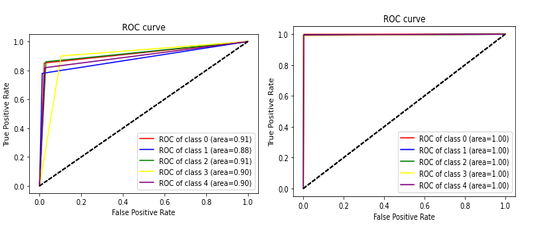
\includegraphics[width=15cm,height=12cm,keepaspectratio]{12.png}
  \caption{نمودار \lr{ROC} برای طبقه بند \lr{SVM}}
  \label{fig:ROCSVM}
\end{figure}

\begin{figure}
  \centering
  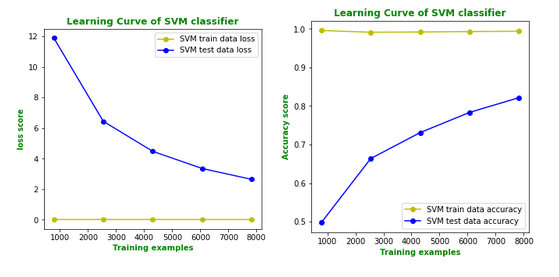
\includegraphics[width=15cm,height=12cm,keepaspectratio]{13.png}
  \caption{نمودار \lr{Learning Curve} برای طبقه بند \lr{SVM}}
  \label{fig:LCSVM}
\end{figure}

\begin{figure}
  \centering
  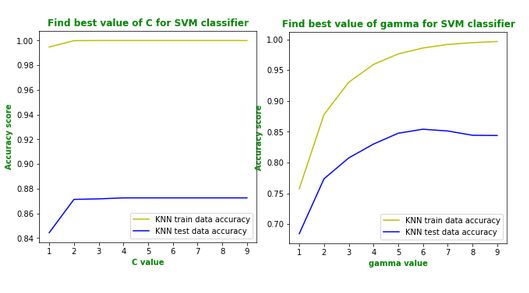
\includegraphics[width=10cm,height=7cm,keepaspectratio]{14.png}
  \caption{نمودار بهترین گاما و \lr{c} برای طبقه بند \lr{SVM}}
  \label{fig:BestGammaSVM}
\end{figure}

همانطور که از نمودار های این بخش هم قابل مشاهده است، دقتی که الگوریتم \lr{SVM} برای داده های آموزش به ما داده است 99.98 درصد و دقتی که برای داده تست به ما داده است حدود 87.13 درصد است. تابع \lr{loss} ای که \lr{SVM} دارد بسیار شبیه به تابع \lr{logistic regression} است.
مشاهده می کنید که مقدار 8 ای که ما برای پارامتر \lr{gamma} مدل خود در نظر گرفتیم، مقدار بهینه برای مدل بود. هر چقدر که بیشتر از این مقدار باشد، با توجه به شیب منحنی، عملکرد مدل کاهش پیدا می کند و مدل دچار \lr{overfitting} می شود. مشاهده می شود که اگر از این مقدار هم کمتر باشد، آنگاه عملکرد مدل روی داده آموزش کاهش می یابد.

برای پارامتر \lr{c} نیز مشاهده می کنید که مقدار 2ای که مدنظر قرار دادیم، مقداری بهینه است و کمتر از این مقدار، عملکرد مدل کاهش می یابد. بیشتر از این مقدار هم تفاوتی برای مدل ندارد. در نتیجه مقدار 2 بین مرز های تصمیم گیری صاف و طبقه بندی صحیح نقاط داده آموزش، تعادل ایجاد می کند. مشاهده می شود که هر چقدر تعداد داده های آموزش و تست افزایش یافته، عملکرد مدل بهتر شده است. دلیل این عملکرد این است که وجود داده های بیشتر منجر به مدل های دقیق تر و بهتر می شود. این کار باعث می شود به جای آنکه به مفروضات و همبستگی های ضعیف تکیه کنیم، به حقایق درست تکیه کنیم. مشاهده می کنیم که با افزایش تعداد داده ها، مقدار \lr{loss} هم کاهش یافته است. یعنی اندازه \lr{margin} بین جداکننده خطی و نزدیک ترین نقاط هر کلاس افزایش یافته و نقاط داده به دلیل اینکه \lr{margin} بهتر انتخاب شده است، توانسته اند بهتر طبقه بندی شوند.


\subsection{طبقه بند \lr{MLP}}
الگوریتم \lr{Multilayer Perceptron Classifier} یکی از ساده ترین الگوریتم های شبکه عصبی است. این نوع از الگوریتم ها بر پایه شبکه های عصبی طبیعی در بدن انسان طراحی شده و شکل گرفته اند.
شبکه‌های عصبی از ساختار مغز انسان الهام گرفته‌اند، اما لزوماً مدل دقیقی از آن نیستند، چرا که هنوز بخش های ناشناخته زیادی از این ساختار برای انسان وجود دارد. اما توانایی و قابلیت زیادی که این شبکه ها در اختیار ما می گذارند، یکی از دلایلی بود که گروه ما را به استفاده از آن ها سوق داد. 

شبکه عصبی \lr{MLP}، یک شبکه عصبی \lr{FeedForward} است؛ یعنی شبکه عصبی بازگشتی ای نیست. در این نوع از شبکه ها دوری میان واحد های تشکیل دهنده شبکه وجود ندارد. جهت این شبکه از سمت نورون ها ورودی به سمت نورون های خروجی و یک طرفه است؛ که در این مسیر از لایه های پنهانی از نورون ها گذر می کنیم. شبکه عصبی ای که ما از آن استفاده می کنیم یک شبکه عصبی با یادگیری نظارت شده است. مسئله بهینه سازی \lr{loss function} در مسئله شبکه عصبی از طریق روش \lr{back propagation} حل شده است. این روش گرادیان تابع هزینه یا همان \lr{loss function} را برای همه وزن های شبکه عصبی حساب می کند و در مرحله بعد از طریق روش گرادیان کاهشی برای پیدا کردن مجموعه وزن های بهینه استفاده می کند. روش گرادیان کاهشی سعی می کند که به صورت متناوب در خلاف جهت اصلی گرادیان حرکت کند و \lr{loss function} را بهینه کند. هدف در این شبکه ها، بهینه کردن تابع هزینه بر روی همه داده ها است.  گرادیان لایه های میانی از روش های مشتق زنجیره ای و گرادیان لایه آخر از روش مشتق جزئی بدست می آید. یک \lr{MLP} حداقل سه لایه دارد، لایه ورودی و لایه پنهان و لایه خروجی. هر کدام از نورون های این شبکه، به جز نورون های لایه ورودی شبکه، از یک \lr{activation function} غیر خطی استفاده می کند.

ما برای طراحی شبکه عصبی پرسپترون خود از \lr{MLPClassifier} کتابخانه \lr{sklearn} استفاده کردیم. ما علاوه بر اینکه دو لایه ورودی و خروجی برای داده های خود داریم، چهار لایه پنهان نیز تعریف کردیم.
تعداد نورون های لایه ورودی متناسب با تعداد فیچر های داده های ورودی ما و تعداد نورون های لایه خروجی نیز متناسب با تعداد برچسب های کلاس های ما هستند؛ که این دو مورد را خود \lr{MLPClassifier}  مدیریت می کند. برای سایر لایه های پنهان شبکه خود نیز، تعداد نورون ها را به صورتی قرار دادیم که شبکه عصبی ما کاهشی باشد؛ یعنی به ترتیب از سمت لایه ورودی به سمت لایه خروجی، 128 نورون و 64 نورون و 32 نورون و 8 نورون برای لایه های پنهان شبکه عصبی خود در نظر گرفتیم. برای الگوریتم خود از \lr{SGD solver} استفاده کردیم.

همانطور که گفته شد، روش گرادیان نزولی، یک الگوریتم بهینه‌سازی است که برای یافتن مقادیر پارامترها یک تابع استفاده می‌شود که تابع هزینه را برای آن به حداقل برساند و بهینه کند هنگامی که پارامترها را نمی توان به صورت تحلیلی و با جبرخطی محاسبه کرد، بهترین راه این است که توسط یک الگوریتم بهینه سازی جستجو شود.

یکی از روش های الگوریتم گرادیان نزولی، روش \lr{batch gradient descent} است. این روش، تمام داده های آموزشی را برای هر تکرار نزول گرادیان، به صورت \lr{batch} به \lr{batch} پردازش می کند. اما اگر تعداد نمونه‌های آموزشی زیاد باشد، از نظر محاسباتی نزول گرادیان دسته‌ای بسیار گران است. طبق الگوریتم زیر، مشاهده می کنید که الگوریتم \lr{BGD} به چه میزان برای داده های زیاد، کند خواهد شد تا به وزن بهینه همگرا شود.

\lr{
\begin{algorithmic}
\Repeat
\State {$\theta_j := \theta_j - \alpha \frac{1}{m} \sum_{i=1}^{m}(h_\theta(x^{(i)})-j^{(i)})x_j^{(i)}$}
\Until{convergence}
\end{algorithmic}
}

از این رو اگر تعداد نمونه های آموزشی زیاد باشد، نزول گرادیان دسته ای ترجیح داده نمی شود؛ (از آنجایی که برای انجام فقط یک به‌روزرسانی باید گرادیان کل مجموعه داده را محاسبه کنیم، نزول گرادیان دسته‌ای می‌تواند بسیار کند باشد و برای مجموعه‌های داده‌ای که در حافظه جا نمی‌شوند، غیر قابل حل است.) و در عوض، ما ترجیح می دهیم از گرادیان نزولی تصادفی یا گرادیان نزولی مینی دسته ای استفاده کنیم.

روش \lr{stochastic gradient descent} بدین صورت عمل می کند که یک نمونه آموزشی را به صورت تصادفی در هر تکرار پردازش می کند. از این رو، پارامترها حتی پس از یک بار تکرار که در آن فقط یک داده پردازش شده است، به روز می شوند. از این رو این بسیار سریعتر از نزول گرادیان دسته ای است. همانطور که گفته شد، این روش از یک داده آموزشی در هر تکرار استفاده می کند که برای مجموعه داده های بزرگ سریعتر از الگوریتم \lr{BGD} است. طبق الگوریتم زیر، مشاهده می کنید که الگوریتم \lr{SGD} به چه صورتی عمل می کند.

\newpage

\lr{
\begin{algorithmic}
\Repeat
\For{$i:=1,...,m$}
    \State {$\theta_j:=\theta_j-\alpha(h_\theta(x^{(i)})-y^{(i)})x_j^{(i)} \hspace{5} (for \hspace{5} every \hspace{5} j = 0,...,n)$} 
\EndFor
\end{algorithmic}
}

در روش گرادیان نزولی تصادفی، ممکن است به وزن بهینه همگرا نشویم، اما محاسبه نتایج سریعتر است؛ بدین صورت که این الگوریتم حول نقطه بهینه هدف برای بهینه سازی تلاش می کند و سعی می کند که به آن نقطه نزدیک تر شود. اما خیلی احتمال آن که به طور دقیق به خود آن نقطه همگرا شود کم است. ولی خیلی به آن نزدیک می شود و حول \lr{global minimum} همگرا می شود. به طور خلاصه، ما یک \lr{trade off} بین استفاده از الگوریتم \lr{BGD} و \lr{SGD} داریم؛ که باید ببینیم زمان برای ما اهمیت بیشتری دارد یا دقت برایمان مهم تر است. در این پروژه، ما ترجیح دادیم که از \lr{SGD} استفاده کنیم. چون به دقت مطلوبی برای مدل خودمی رسیدیم و ترجیح می دادیم که از لحاظ زمانی هم مدل ما بهینه تر باشد.

برای مدل خود از \lr{batch size} برابر 32 استفاده کردیم و تعداد بیشینه \lr{epoch} را برابر 350 قرار دادیم.
اندازه دسته ای یک هایپرپارامتر است که تعداد نمونه هایی را که باید قبل از به روز رسانی پارامترهای مدل کار کنند را تعیین می کند. بدین صورت که از هر دسته، یک نمونه برای الگوریتم \lr{SGD} انتخاب می شود؛ پس اندازه آن را باید طوری انتخاب کنیم که الگوریتم \lr{SGD} به صورت بهینه عمل کند.
تعداد دوره های تکرار آموزش مدل یا \lr{epoch} یک هایپرپارامتر است که تعداد دفعات تکراری را که الگوریتم یادگیری مدل روی مجموعه داده آموزشی کار می کند را تعیین می کند. یک دوره از یک یا چند \lr{batch} تشکیل شده است. تعداد دوره‌ها معمولاً زیاد است، که به الگوریتم یادگیری مدل اجازه می‌دهد تا زمانی که خطای مدل به اندازه کافی بهینه شود، تکرار و اجرا شود. معمولاً آموزش مدل روی داده های آموزشی، تا قبل از زمانی که مدل ما \lr{overfit} کند، ادامه پیدا می کند. یک روش این است که الگوریتم را تا زمانی که امکان دارد اجرا کنیم (یعنی تعداد دوره های تکرار را زیاد قرار دهیم.) و با استفاده از معیاری مانند تغییر (یا عدم تغییر) در خطای مدل در طول دوره ها، آموزش را متوقف کنیم؛ که ما یه همین دلیل تعداد دوره ها را طوری قرار دادیم که الگوریتم تا حد ممکن اجرا شود و هایپرپارامتر ها را بهینه کند.

ما برای مدل خود، یک \lr{random state} هم تنظیم کردیم. این کار باعث می شود که مقادیر اولیه وزن های شبکه و مقدار اولیه بایاس و دیتاهای درون هر \lr{batch} به صورت رندوم و تصادفی انتخاب شوند و این به یادگیری بدون جهت مدل ما کمک می کند(شکل \ref{fig:ROCMLP} های ، \ref{fig:LCMLP} و \ref{fig:LossMLP}).

ما مقدار \lr{learning rate} را برابر 0.01 قرار دادیم. نرخ یادگیری سرعت آموزش مدل را کنترل می کند. و این پارامتر ممکن است مهمترین هایپر پارامتر برای مدل باشد. هر چه مقدار \lr{rate} سرعت تمرین بیشتر باشد، وزن ما سریع تر و بیشتر تغییر می کند و این باعث می شود مدل ما نامرئی شود. و هر چه این سرعت یادگیری کمتر باشد، وزن کم و کمتر می شود و ممکن است روی دقت خاصی و مینیمم محلی گیر کرده و به روز رسانی متوقف شود؛ پس باید یک مقدار مناسب برای آن انتخاب کنیم.
به طور کلی، ما از بهینه ساز ها برای بهینه سازی و رفع مشکلات احتمالی در طول عملیات آموزش شبکه عصبی استفاده می کنیم. مومنتوم پارامتری مانند پارامتر نرخ یادگیری است.
از آنجایی که داده‌های ما حاوی داده‌های نویز هستند، ممکن است در به‌روزرسانی وزن‌ها اشتباه کنیم و در حداقل‌های محلی گیر کنیم و آموزش شبکه متوقف شود. این پارامتر به عبور از حداقل های محلی برای ادامه پیشرفت آموزش شبکه کمک می کند. مقدار کم پارامتر مومنتوم باعث می شود که آموزش شبکه دوباره با مشکل مواجه شود و در حداقل های محلی گرفتار شود و از آنها عبور نکند. و مقدار زیاد برای پارامتر مومنتوم سرعت به روز رسانی وزن ها را افزایش می دهد و ما را از نتیجه مطلوب و بهینه دور می کند و به جای پرش از روی حداقل های محلی، از روی وزن های ایده آل می پرد.


\begin{figure}
  \centering
  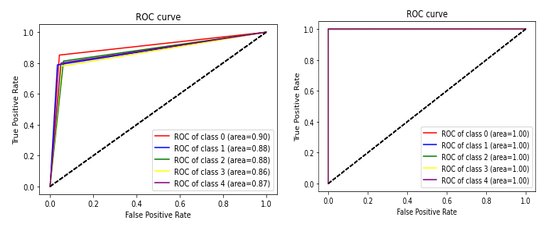
\includegraphics[width=10cm,height=7cm,keepaspectratio]{15.png}
  \caption{نمودار \lr{ROC} برای طبقه بند \lr{MLP}}
  \label{fig:ROCMLP}
\end{figure}

\begin{figure}
  \centering
  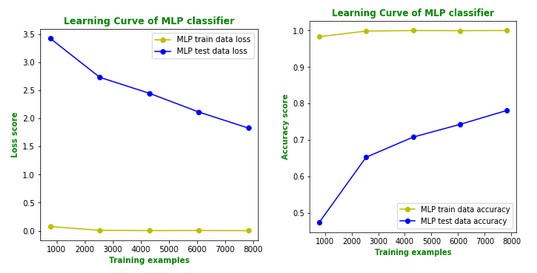
\includegraphics[width=10cm,height=7cm,keepaspectratio]{16.png}
  \caption{نمودار \lr{Learning Curve} برای طبقه بند \lr{MLP}}
  \label{fig:LCMLP}
\end{figure}

\begin{figure}
  \centering
  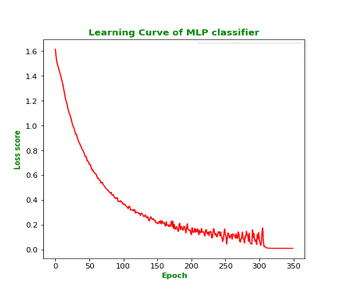
\includegraphics[width=10cm,height=7cm,keepaspectratio]{17.png}
  \caption{نمودار تغییرات \lr{loss} به ازای \lr{epoch} برای طبقه بند \lr{MLP}}
  \label{fig:LossMLP}
\end{figure}

همانطور که از نمودار های این بخش هم قابل مشاهده است، دقتی که الگوریتم \lr{MLP} برای داده های آموزش به ما داده است 99.97 درصد و دقتی که برای داده تست به ما داده است حدود 80.67 درصد است. مشاهده می شود که هر چقدر تعداد داده ها افزایش یافته است، دقت و عملکرد مدل بهتر شده است. برای بهبود عملکرد شبکه، ما تعداد لایه های پنهان را بیشتر کردیم؛ چون بسیاری از توابع و مدل ها در سطح بالاتری از انتزاع همگرا خواهند شد. در این لایه های پنهان اگر تعداد ناکافی نورون استفاده شود، شبکه قادر به مدل سازی داده های پیچیده نخواهد بود و تناسب حاصله ضعیف خواهد بود؛ و اگر از تعداد زیادی نورون استفاده شود، زمان آموزش ممکن است بیش از حد طولانی شود، و بدتر از آن، شبکه ممکن است بیش از حد بر روی داده ها آموزش ببیند و \lr{overfit} کند. در نتیجه تعداد نورون ها را هم بهینه انتخاب کردیم. و اینکه وقتی داده های زیادی داریم، شبکه عصبی به خوبی تعمیم می یابد. در غیر این صورت، اگر داده ها کم باشد، ممکن است مدل دچار \lr{overfitting} شود. در نمودار \lr{loss} بر حسب تعداد داده هم مشاهده می کنید که وقتی تعداد داده ها بیشتر می شود مدل بهتر تعمیم می باید و خطای آموزشش کاسته می شود. در نمودار \lr{loss} بر حسب \lr{epoch} هم مشاهده می کنید که هر چقدر \lr{epoch} ها افزایش یافته و مدل تعداد دفعات بیشتری روی داده آموزش یافته و وزن بهینه تری پیدا کرده، خطای مدل کاهش یافته است.

\section{خوشه بندی}
خوشه بندی، وظیفه نقاط داده به تعدادی کلاس است؛ به طوری که نقاط داده در همان گروه کلاس ها بیشتر شبیه سایر نقاط داده در همان گروه باشد تا اینکه به سایر گروه ها شبیه باشد. پس هدف، تفکیک کلاس هایی با صفات مشابه و تخصیص آن ها به خوشه‌ها است.

انواع مختلفی از الگوریتم های خوشه بندی وجود دارد؛ یک نوع آن \lr{Connectivity} مدل ها هستند. این مدل‌ها بر اساس این هستند که در فضای داده ها، نقاط داده نزدیک‌تر شباهت بیشتری به یکدیگر نسبت به نقاط داده دورتر دارند. در یک رویکرد، آن ها با طبقه‌بندی تمام نقاط داده در خوشه‌های جداگانه و سپس جمع‌آوری آن ها با کاهش فاصله است. در رویکرد دیگری، تمام نقاط داده به عنوان یک خوشه طبقه بندی می شوند و سپس با افزایش فاصله، تقسیم بندی می شوند.این مدل ها، برای مجموعه داده های بزرگ، به خوبی کار نمی کنند. نمونه هایی از این مدل ها، الگوریتم خوشه بندی \lr{hierarchical} است. نوع دیگر این الگوریتم ها، \lr{Centroid} مدل ها هستند. این ها الگوریتم‌های خوشه‌بندی \lr{iterative} هستند (تکرار چند باره برای پیدا کردن بهینه محلی) که مفهوم شباهت در آن ها، از نزدیکی یک نقطه داده به مرکز خوشه‌ به دست می‌آید. الگوریتم خوشه بندی \lr{K-Means} در این دسته قرار می گیرد. در این مدل ها، تعداد خوشه های مورد نیاز باید از قبل مشخص باشد. مدل دیگر الگوریتم های خوشه بندی، مدل \lr{Distribution} است. این خوشه‌بندی مبتنی بر این است که احتمال تعلق همه نقاط داده در خوشه را به یک توزیع مثل توزیع گاوسی بررسی می کند. الگوریتم خوشه بندی \lr{EM}، در این دسته قرار می گیرد. این مدل الگوریتم ها احتمال آنکه با مشکل \lr{overfitting} رو به رو شوند، زیاد است. مدل آخر خوشه بندی، مدل \lr{Density} است. این مدل‌ها نواحی مختلف چگال تر فضای داده ها را جدا می کند و نقاط داده ها در این مناطق را به یک خوشه اختصاص می دهد.

\subsection{خوشه بندی \lr{K Means}}
الگوریتم \lr{K mean} یک الگوریتم خوشه‌بندی \lr{iterative} است که هدف آن یافتن ماکزیمم محلی در هر تکرار است. این الگوریتم بدین صورت عمل می کند که در ابتدا تعداد خوشه هدف را مشخص می کنیم؛ سپس به طور تصادفی هر نقطه داده را به یک خوشه اختصاص داده می شود. سپس مراکز خوشه ها را حساب می کنیم. بعد هر نقطه را به نزدیکترین مرکز خوشه اش تخصیص می دهیم و به محاسبه مجدد مرکزهای خوشه ای می پردازیم. سپس دو مرحله آخر را به صورت تکراری محاسبه و اجرا می کنیم. زمانی که دیگر نقاط داده بین دو خوشه برای دو تکرار متوالی تغییر نکند، آنگاه پایان الگوریتم را اعلام می کنیم.

این الگوریتم، الگوریتم سریعی است؛ با این حال، عملکرد آن معمولاً به اندازه سایر تکنیک‌های خوشه‌بندی نیست، چون تغییرات جزئی در داده‌ها می‌تواند منجر به واریانس بالا در مدل شود. علاوه بر این، خوشه‌ها کروی و با اندازه یکنواخت فرض می‌شوند، که همین موضوع امکان دارد که عملکرد مدل را کاهش دهد.

ما در این قسمت، از الگوریتم \lr{KMeans} از کتابخانه \lr{sklearn} استفاده کردیم.
تعداد \lr{n\_cluster} را بین 2 تا 5 متغیر گذاشتیم و الگوریتم را تکرار کردیم. الگوریتم بدین صورت عمل می کند که تعداد \lr{n\_cluster} را دریافت می کند و به همین تعداد مرکز خوشه حساب می کند و داده ها را هم بین همین خوشه ها تقسیم می کند.

ما الگوریتم \lr{init} را برابر \lr{"++ k-means"} قرار دادیم؛ از آنجایی که هدف خوشه‌بندی \\ \lr{k-means} بر روی مجموعه بهینه‌ای از مراکز خوشه و عضویت داده ها در خوشه بر اساس فاصله از این مرکزها از طریق تکرارهای متوالی است، هر چه موقعیت‌ این مرکزهای اولیه بهینه‌تر باشد، تکرارهای کمتری لازم خواهد بود. پس برخی از ملاحظات برای شروع اولیه این مرکزهای اولیه می تواند مفید باشد. این الگوریتم، مرکز اول را به طور تصادفی محل یک نقطه داده انتخاب می کند؛ و سپس مرکز های بعدی را از بین نقاط داده باقی مانده بر اساس احتمالی متناسب با مجذور فاصله نقطه داده شده از نزدیکترین مرکز موجود انتخاب می کند.

ما برای مدل خود، یک \lr{random state} هم تنظیم کردیم. این کار باعث می شود که هایپرپارامتر های اولیه به صورت رندوم و تصادفی انتخاب شوند و این به یادگیری بدون جهت مدل ما کمک می کند.
ما \lr{max\_iter} را هم برابر 100 قرار دادیم. این هایپرپارامتر تعداد اجرای الگوریتم را مشخص می کند. ما از الگوریتم \lr{elkan} (بر پایه نابرابری مثلث) هم در مدل خود استفاده کردیم تا محاسبات فاصله برای خوشه بندی داده ها کاهش بیابد(شکل \ref{fig:KMeans}).

\begin{figure}
  \centering
  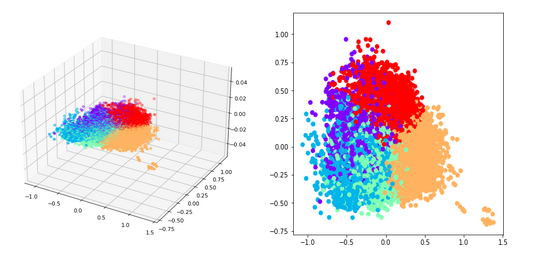
\includegraphics[width=10cm,height=7cm,keepaspectratio]{18.png}
  \caption{خوشه بندی توسط \lr{KMeans}}
  \label{fig:KMeans}
\end{figure}

همانطور که از شکل ها مشخص است می توان گفت که داده ها از کلاس های مختلف با هم همپوشانی زیادی دارند؛ بدین صورت که 4 کلاس از 5 تا کلاس هدف، به خوبی خوشه بندی شده اند و یک کلاس دیگر قدری ضعیف تر خوشه بندی شده است و با دو تا از خوشه ها همپوشانی دارد. حدس ما این است که داده های کلاس های بندری و گیلکی بهتر از سایر داده ها خوشه بندی می شوند و داده های سه کلاس دیگر، همپوشانی بیشتری دارند و احتمالاَ داده های کلاس لری با داده های کلاس کردی و ترکی شباهت بیشتری به نسبت سایر لیبل ها دارد و داده های کلاس ترکی و کردی به نسبت همدیگر بهتر خوشه بندی شده اند. در حالتی که 2 کلاستر برای خوشه بندی داریم از حالت 5 کلاستر، بهتر نتیجه گرفتیم. علت آن می تواند این باشد که داده های ما همپوشانی زیادی با هم دارند و جداسازی آن ها به سادگی امکان پذیر نیست. در نتیجه داده هایی که ممکن است در یکی از این دو کلاستر قرار بگیرند ممکن است شباهت بیشتری نسبت به حالت سه کلاستر و چهار کلاستر، به هم داشته باشند. ولی همانطور هم که انتظار داشتیم خوشه بندی با 5 کلاستر نتیجه بهتری نسبت به سایر حالت ها داده است. (عملکرد حالت دو کلاستر هم خیلی تفاوت چندانی با حالت پنج کلاستر ندارد.)

\subsection{خوشه بندی \lr{DBSCAN}}
ایده اصلی پشت الگوریتم \lr{DBSCAN} این است که یک نقطه به یک خوشه تعلق دارد اگر به نقاط زیادی از آن خوشه نزدیک باشد. بنابراین این الگوریتم می تواند خوشه های با شکل دلخواه و خوشه های دارای داده های نویزی را پیدا کند. 

بدین صورت عمل می کنیم که بر اساس چگالی نقاط در یک محدوده فضای نقاط داده، داده ها را خوشه خوشه می کنیم. مرز بین خوشه های مختلف را کم شدن چگالی بین دو منطقه چگال مشخص می کند.

در این الگوریتم هم برای محاسبه شباهت دو نقطه نسبت به هم از متریک فاصله استفاده می شود و هر چقدر که دو نقطه به هم نزدیک تر باشند، شبیه تر خواهند بود.

مزیت این روش به نسبت روش‌ های دیگری خوشه‌بندی مانند \lr{KMeans} این است که نسبت به شکل داده‌ها حساس نمی‌باشد و می‌تواند اشکال غیر منظم را نیز در داده‌ها تشخیص دهد.

دو هایپر پارامتر \lr{DBSCAN} پارامتر \lr{eps} و پارامتر \lr{minPts} است.پارامتر اول، مناطق را مشخص می کند. اگر فاصله بین نقاط فضای داده، کمتر یا مساوی با \lr{eps} باشد، دو نقطه همسایه و در یک خوشه در نظر گرفته می شوند. پارامتر دوم نیز حداقل تعداد نقاط داده برای تعریف یک خوشه را مشخص می کند. بر اساس این دو پارامتر، نقاط فضای داده به عنوان نقطه هسته، نقطه مرزی یا نقطه پرت طبقه بندی می شوند؛ که یک نقطه یک نقطه هسته است اگر حداقل به تعداد \lr{MinPts} نقطه (از جمله خود آن نقطه) در ناحیه اطراف آن نقطه با شعاع \lr{eps} وجود داشته باشد. و نقطه ای یک نقطه مرزی است که از یک نقطه مرکزی به شعاع \lr{eps} قابل دسترسی باشد و تعداد نقاطی کمتر از \lr{MinPts} در محدوده اطراف آن نقطه وجود داشته باشد. (یعنی که آن نقطه، خود مرکز نباشد.) و در آخر نقطه ای نقطه پرت است که نقطه مرکزی نباشد و از هیچ نقطه مرکزی هم قابل دسترسی نباشد. نقطه‌ای که به‌عنوان نویز مشخص شده است، ممکن است دوباره بررسی شود و بخشی از یک خوشه قرار بگیرد. در هر مرحله به طور تصادفی نقطه دیگری از بین نقاطی که در مراحل قبل بازدید نشده است را انتخاب و خوشه بندی می کنیم. این فرآیند با بازدید از تمام نقاط فضای داده، به پایان می رسد.

با اعمال این مراحل، الگوریتم \lr{DBSCAN} قادر است مناطق با چگالی بالا را پیدا کرده و آنها را از مناطق کم تراکم جدا کند. یک خوشه شامل نقاط مرکزی است که همسایه هستند (یعنی قابل دسترسی از یکدیگر هستند.) و تمام نقاط مرزی با این نقاط اصلی را هم شامل می شوند. شرط لازم برای تشکیل یک خوشه، داشتن حداقل یک نقطه مرکزی است.

ما از الگوریتم \lr{DBSCAN} از کتابخانه \lr{sklearn} استفاده کردیم. مقدار پارامتر \lr{eps} را برابر 0.8 قرار دادیم. سپس \lr{min\_samples} که همان \lr{MinPts} است را برابر 3 قرار دادیم. برای فاصله هم از متریک \lr{manhattan} استفاده کردیم. و \lr{n\_jobs} را برابر 2 قرار دادیم که تعداد کار های موازی قابل اجرا را مشخص می کند(شکل \ref{fig:DBSCAN}).

\begin{figure}
  \centering
  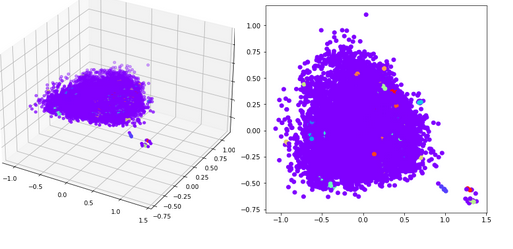
\includegraphics[width=10cm,height=7cm,keepaspectratio]{20.png}
  \caption{خوشه بندی توسط \lr{DBSCAN}}
  \label{fig:DBSCAN}
\end{figure}

دقتی که از الگوریتم \lr{DBSCAN} گرفتیم به نسبت دو الگوریتم کلاسترینگ دیگر تغییر خاصی نداشت. این الگوریتم بر اساس چگالی نقاط فضای داده، داده ها را خوشه بندی می کند. از آن جایی که داده های ما با هم همپوشانی زیادی دارند، ممکن است بر اساس چگالی نتوان به خوبی دو الگوریتم دیگر استفاده شده در این پروژه خوشه بندی کرد. همانطور که از دو شکل این قسمت هم قابل مشاهده است، یک خوشه بزرگ که شامل فضای چگال تر از کل فضای داده ما است، تشکیل شده است و بیشتر داده های ما در این خوشه قرار گرفته اند. علت این موضوع می تواند این باشد که همه داده های صوتی ما از یک زبان یک کشور هستند.

\subsection{خوشه بند \lr{K Medoids}}

ایده خوشه‌بندی \lr{K-Medoids} این است که مرکز های نهایی را نقاط داده واقعی فرض کنیم. این نتیجه باعث می شود که مرکز های خوشه ها قابل تفسیر شوند. یک مشکل در خوشه بندی \lr{K-Means} این است که مرکزهای نهایی قابل تفسیر نیستند یا به عبارت دیگر، مرکز ها نقطه واقعی نیستند بلکه میانگین نقاط موجود در آن خوشه هستند. در \lr{K-medoids Clustering}، به جای اینکه مرکز داده ها در یک خوشه را به عنوان نقطه مرکزی در نظر بگیریم، \lr{medoid} را به عنوان نقطه مرکزی در نظر می گیریم. نقطه \lr{medoid} مرکزی ترین داده در یک خوشه است که میانگین تفاوت آن با همه داده های خوشه کمینه است. بنابراین، الگوریتم \lr{K-medoids} نسبت به الگوریتم \lr{K-means} نسبت به داده های نویزی قوی تر است.

ما در این قسمت، از الگوریتم \lr{KMedoids} از کتابخانه \lr{sklearn} استفاده کردیم.
تعداد \lr{n\_cluster} را بین 2 تا 5 متغیر گذاشتیم و الگوریتم را تکرار کردیم. الگوریتم بدین صورت عمل می کند که تعداد \lr{n\_cluster} را دریافت می کند و به همین تعداد مرکز خوشه حساب می کند و داده ها را هم بین همین خوشه ها تقسیم می کند.

همچنین از متریک \lr{pam} یا \lr{partition around medoids} استفاده کردیم. از آنجایی که خوشه بندی را بر روی داده های کلی و نه فقط بر روی نمونه های انتخاب شده از مجموعه داده ها انجام می دهد، از این رو، برای مجموعه داده های بزرگ کارآمد نیست. البته \lr{pam} پرهزینه هم است؛ زیرا خوشه بندی را روی مجموعه داده های کلی انجام می دهد.

ما الگوریتم \lr{init} را برابر \lr{"++ k-medoids"} قرار دادیم؛ این الگوریتم هم از رویکردی مبتنی بر الگوریتم \lr{"++ k-means"} پیروی می کند و به طور کلی، \lr{medoid} های اولیه را ارائه می دهد که از روش های دیگر جدا تر هستند. از آنجایی که هدف خوشه‌بندی \lr{k-medoids} بر روی مجموعه بهینه‌ای از \lr{medoid} ها است و عضویت داده ها در خوشه بر اساس فاصله از این \lr{medoid} ها از طریق تکرارهای متوالی است، هر چه موقعیت‌ این \lr{medoid} های اولیه بهینه‌تر باشد، تکرارهای کمتری لازم خواهد بود. 
ما برای مدل خود، یک \lr{random state} هم تنظیم کردیم. این کار باعث می شود که هایپرپارامتر های اولیه به صورت رندوم و تصادفی انتخاب شوند و این به یادگیری بدون جهت مدل ما کمک می کند.
ما \lr{max\_iter} را هم برابر 100 قرار دادیم. این هایپرپارامتر تعداد اجرای الگوریتم را مشخص می کند.
در این الگوریتم در ابتدا \lr{k} تا خوشه مشخص می کنیم. سپس به طور تصادفی \lr{k} داده را از فضای داده ها انتخاب کرده و به \lr{k} تا خوشه مذکور نسبت می دهیم. این \lr{k} داده که هر کدام باید به یک خوشه اختصاص داده شوند، هر کدام یک \lr{medoid} اولیه برای آن خوشه خواهند شد. حال برای همه نقاط داخل فضای داده ها، فاصله های آن ها را از \lr{medoid} ها محاسبه می کنیم و هر نقطه را به خوشه دارای نزدیکترین \lr{medoid} نسبت می دهیم. حال هزینه کل را طبق فاصله ها محاسبه می کنیم و بعد یک داده رندوم را انتخاب می کنیم و تا یک \lr{medoid} دیگر هزینه اش را محاسبه می کنیم. اگر هزینه جدید از هزینه قبلی آن داده کمتر بود، خوشه آن داده را تغییر می دهیم. این عملیات را به صورت تکراری اجرا می کنیم تا وقتی که دیگر خوشه بندی داده ها تغییر نکند(شکل \ref{fig:KMedoids}).

\begin{figure}
  \centering
  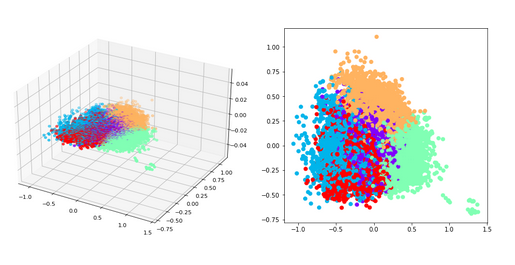
\includegraphics[width=10cm,height=7cm,keepaspectratio]{19.png}
  \caption{خوشه بندی توسط \lr{K Medoids}}
  \label{fig:KMeans}
\end{figure}

همانطور که از شکل های بالا مشاهده می شود خوشه بندی این الگوریتم تفاوت چندانی با خوشه بندی \lr{KMeans} ندارد. همانطور که از شکل ها مشخص است می توان گفت که داده ها از کلاس های مختلف با هم همپوشانی زیادی دارند؛ بدین صورت که 3 کلاس از 5 تا کلاس هدف، به خوبی خوشه بندی شده اند و یک کلاس دیگر قدری ضعیف تر خوشه بندی شده است و با دو تا از خوشه ها همپوشانی دارد. در این الگوریتم هم در حالت خوشه بندی با دو خوشه، اندکی بهتر از حالت پنج خوشه نتیجه گرفتیم که مانند قبل می توان آن را توجیه کرد.


\section{نتایج}

نتایج طبقه بند ها و خوشه بند ها بر اساس پارامتر های یاد شده در بخش های قبل در جداول 1 و 2 آمده است.

\begin{table}[!h]
  \centering
  \caption{نتایج طبقه بند ها}
	\begin{tabular}{|c|c|c|c|c|r|}
	\hline
		 \lr{ROC area} & \lr{f1} & \lr{precision} & \lr{recall} & \lr{accuracy} & \\
	\hline
		 \lr{1} & \lr{1} & \lr{1} & \lr{1} & \lr{1} & \lr{KNN train} \\
	\hline
		 \lr{0.94} & \lr{0.91} & \lr{0.91} & \lr{0.91} & \lr{0.9089} & \lr{KNN test} \\
    \hline
		 \lr{1} & \lr{1} & \lr{1} & \lr{1} & \lr{0.9998} & \lr{SVM train} \\
    \hline
		 \lr{0.92} & \lr{0.87} & \lr{0.87} & \lr{0.88} & \lr{0.8713} & \lr{SVM test} \\
	\hline
		 \lr{1} & \lr{1} & \lr{1} & \lr{1} & \lr{0.9997} & \lr{MLP train} \\
	\hline
		 \lr{0.88} & \lr{0.81} & \lr{0.81} & \lr{0.81} & \lr{0.8067} & \lr{MLP test} \\
	\hline		 
	\end{tabular} 
\end{table}

\begin{table}[!h]
  \centering
  \caption{\lr{silhouette\_score} بر روی  خوشه بند ها}
	\begin{tabular}{|c|c|c|c|r|}
	\hline
		 \lr{5 cluster} & \lr{4 cluster} & \lr{3 cluster} & \lr{2 cluster} & \\
	\hline
		 \lr{0.5337} & \lr{0.4938} & \lr{0.4756} & \lr{0.5608} & \lr{KMeans train} \\
	\hline
		 \lr{0.5624} & \lr{0.4784} & \lr{0.4980} & \lr{0.5379} & \lr{KMeans test} \\
    \hline
		 \lr{0.5337} & \lr{0.5337} & \lr{0.5337} & \lr{0.5337} & \lr{DBSCAN train} \\
    \hline
		 \lr{0.5379} & \lr{0.5379} & \lr{0.5379} & \lr{0.5379} & \lr{DBSCAN test} \\
	\hline
		 \lr{0.5608} & \lr{0.4559} & \lr{0.4896} & \lr{0.53737} & \lr{KMedoids train} \\
	\hline
		 \lr{0.5608} & \lr{0.4557} & \lr{0.4937} & \lr{0.5379} & \lr{KMedoids test} \\
	\hline		 
	\end{tabular} 
\end{table}

\end{document}